\chapter{Proof-of-Concept}

\section{Systemübersicht}
Das Proof-Of-Concept als Umsetzung beinhaltet die Logik und Kommunikation zwischen dem Gestensensor und der Drohne über die jeweils bestehenden \gls{apiLabel}'s.

Folglich sind die zwei Hauptkomponenten der Umsetzung der \textit{Crazyflie Controller} (\secref{sec:poc:controllerCrazyflie}) und der \textit{Detection Controller} (\secref{sec:poc:controllerDetection}).

\subsection{Crazyflie Controller}
\label{sec:poc:controllerCrazyflie}
Der Crazyflie Controller stellt die Verbindung zur Drohne her, durch die Steuerkommandos übermittelt werden können.
Dabei stellt das Management der Verbindung den Hauptteil des Codes dieses Controlles dar.
Beim Verbindungsaufbau, sowie bei erfolgreicher Verbindung müssen mögliche Fehler-Events abgefangen werden und der Zustand der Verbindung muss gegen aussen abrufbar sein.
Ansonsten hat der Crazyflie Controller keine Aufgabe.

\subsection{Detection Controller}
\label{sec:poc:controllerDetection}
Der Detection Controller bildet den Kern der Applikation. Er kommuniziert mit dem Leap Motion, erhält die Gesten Informationen, wertet diese abhängig des Zustandes der Steuerung aus und definiert daraus die Kommandos die via den Crazyflie Controller der Drohne übermitteln werden sollen.
Die ganze Logik der Steuerung findet sich dementsprechend in diesem Teil.

Um die Auswertung der Gesten abhängig des Zustandes angemessen aufzuteilen, gibt es für jeden Zustand einen eigenen \textit{State Handler}.

\clearpage

\subsection{Datei Struktur}
\begin{wrapfigure}{l}{0.4\textwidth}
	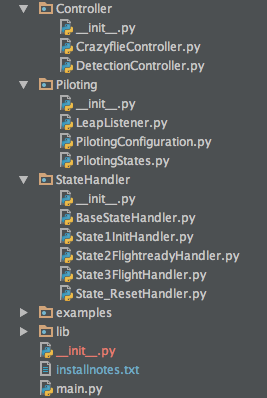
\includegraphics[width=1.0\linewidth]{figures/poc/filestructure.png}
	\caption[Dateistruktur]{Dateistruktur der Umsetzung}
\end{wrapfigure}
Die gesamte Umsetzung im Verzeichnis \textit{code} besteht aus drei Modulen und ist wie folgt aufgegliedert:

\subsubsection{Controller}
Die Controllers wurden bereits oben erwähnt. Jeder Controller trägt die Verantwortung einer Komponenten (Detection via Leap Motion oder Crazyflie).
Nach dem Aufruf eines Controllers, übernimmt ein Controller die Kommunikation und Verwaltung der zugeordneten Komponente.

Um die Controller schlank zu halten, greifen die Controller auf Code aus weiteren Modulen (\textit{Piloting} und \textit{StateHandler}) zu.
Um eine Komponente via \gls{apiLabel} zu verwenden, sind werden oft folgende Schritte benötigt.
Die Verbindung zur Komponente muss aufgebaut werden, und kann über verschiedene Parameter konfiguriert werden.
Zudem können diverse Callback-Events registriert werden, die von der Komponente bei bestimmten Ereignissen aufgerufen werden können (Beispiele sind: erfolgreiche Verbindung, Verbindungsunterbruch, sowie auch konkrete Daten die zur Verfügung stehen wie erkannte Gesten vom LeapMotion).

\subsubsection{StateHandler}
Jeder Status in den die Drohne versetzt werden kann, wird durch einen eigenen \textit{StateHandler} abgebildet.
Ein \textit{StateHandler} hat Zugriff auf die Gesteninformationen und wertet diese gemäss den statusabhängigen Möglichkeiten aus.
Wird der Status (\textit{next\_state}) geändert, wird beim nächsten verfügbaren Frame jener \textit{StatusHandler} aufgerufen.

In der vorliegenden Umsetzung gibt es die folgenden \textit{StateHandlers}:
\begin{itemize}
	\item State1InitHandler
	\item State2FlightreadyHandler
	\item State3FlightHandler
	\item State\_ResetHandler
\end{itemize}
Alle \textit{StateHandler} erben von der \textit{BaseStateHandler}-Klasse, welche die grundsätzlich verfügbaren Variablen (erkannte Gesten, Crazyflie, und den eigenen sowie den nächsten Status) definiert.

\subsubsection{Piloting}
Das Modul Piloting beinhaltet allgemeine steuerspezifische Konfigurationen.
Dazu gehört die Verknüpfung zwischen Status Nummer, Status Bezeichnung und dem jeweiligen StateHandler, so wie auch verschiedne Flugparameter (z.B.: maximaler Power).

Nebst der Konfiguration beinhaltet das \textit{Piloting} Modul einen \textit{LeapListener} der die notwendigen Callbacks für den Leap Motion Sensor registriert. Darunter die Funktion \textit{on\_frame()} die bei jedem erkannten Frame aufgerufen wird.
Es befindet sich aber keinen Status spezifischen Code im \textit{Piloting}.

\section{Anpassungen am Konzept}
\label{sec:poc:conceptChanges}
Die ursprüngliche Steuerung (gemäss \secref{sec:concept:stateoverview}) wurde während der Umsetzung optimiert.

Das Zustands-Diagramm wurde wie folgt angepasst:
\begin{figure}[H]
	\centering
	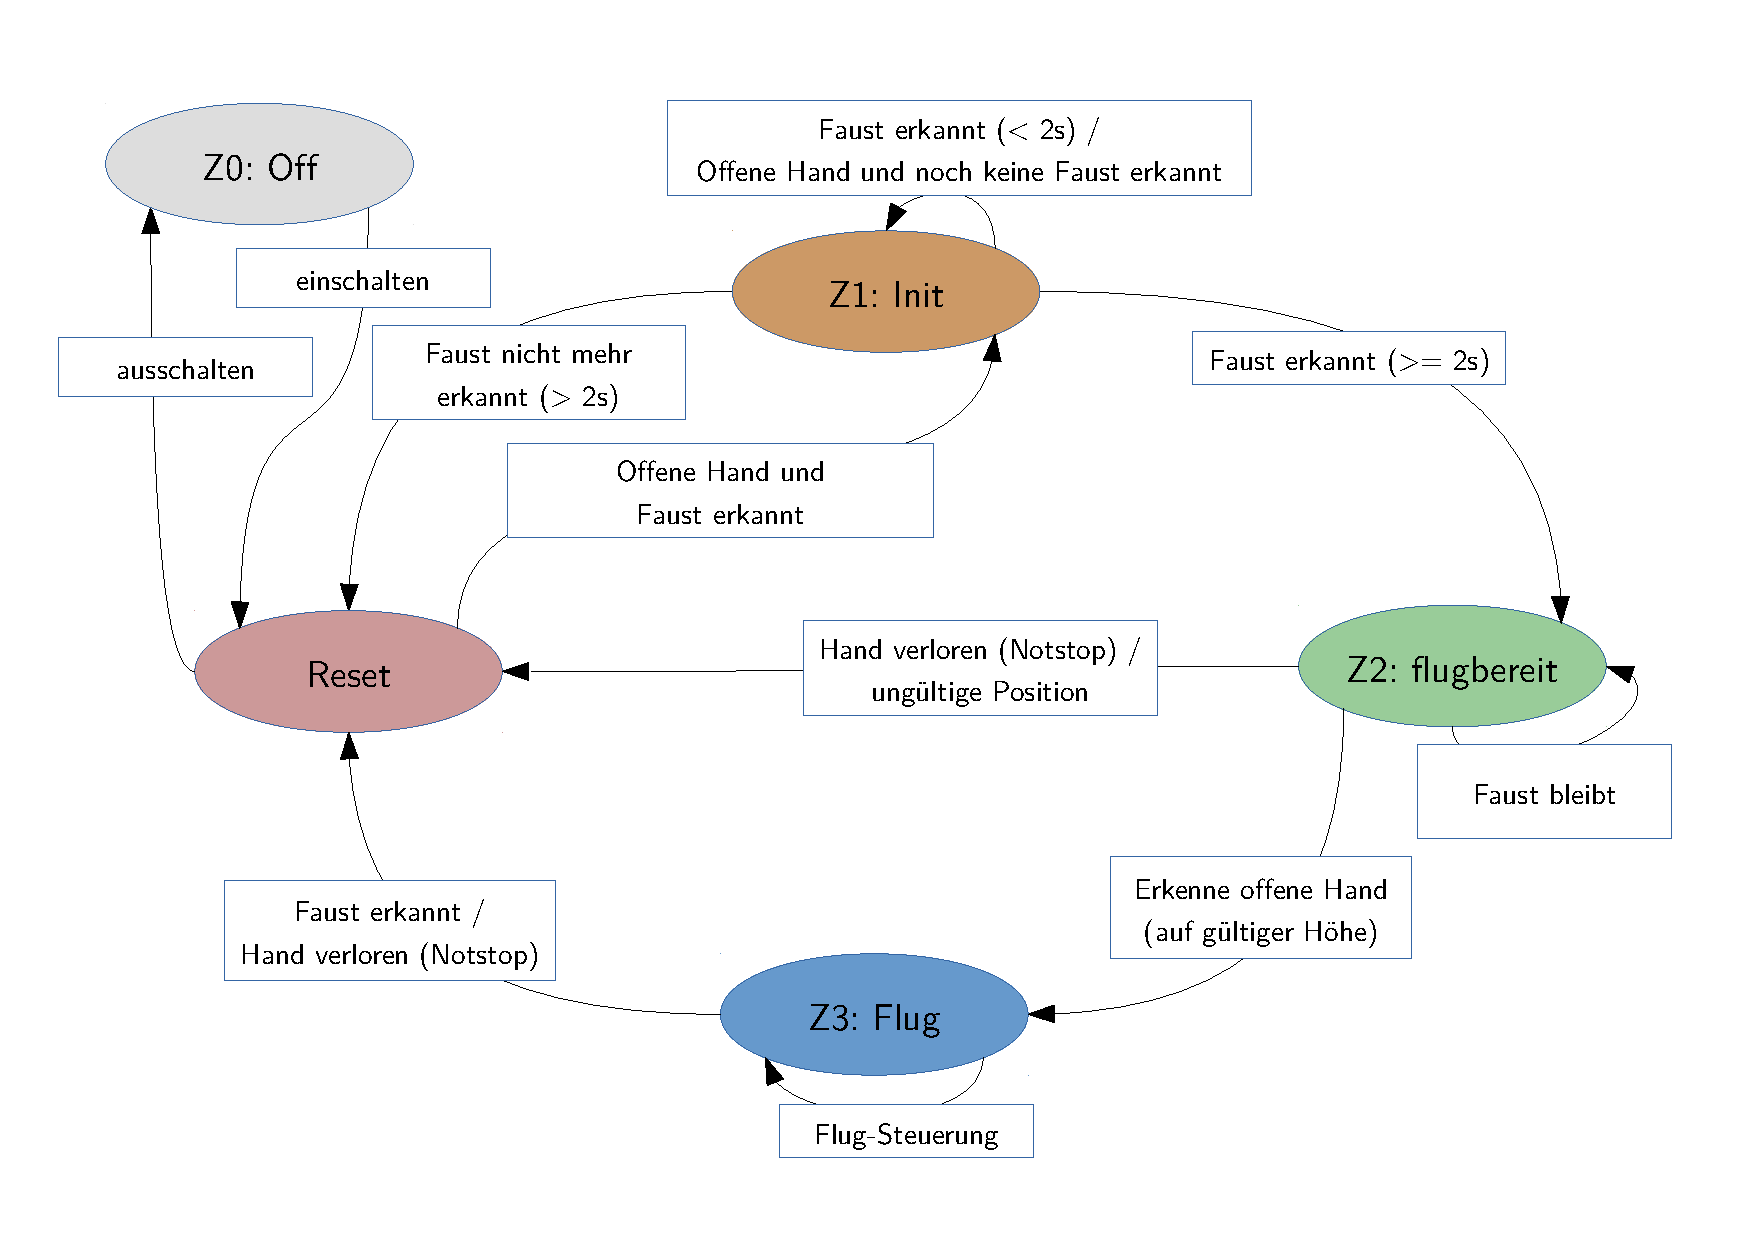
\includegraphics[width=1.0\textwidth]{figures/concept/state-diagram-2.pdf}
	\caption[Zustands-Diagramm: Drohne mit optimierter Gestensteuerung optimiert]{Zustands-Diagramm: Drohne mit optimierter Gestensteuerung}
	\label{key}
\end{figure}

Folgend werden die durchgeführten Änderungen erläutert und begründet.

\subsection{"'Z4: unkontrolliert"' entfernt}
Der Zustand \textit{Z4: unkontrolliert} wurde entfernt.
Diverse Testflüge zeigten auf, dass die Verbindung zur Drohne, so wie auch zum Leap Motion sehr stabil läuft und daher keine unerwartete Unterbrüche zu überbrücken sind.

Gleichzeitig wurde ein neues Bedürfnis des Piloten erkannt: die Drohne bei kritischen Flugsituationen möglich rasch stoppen zu können, resp. die Rotoren auszuschalten.
So kann Schaden an den Rotoren vermieden werden, welche gewöhnlicherweise am häufigsten ersetzt werde müssen.
Auch können andere Gegenstände durch die drehenden Rotoren beschädigt werden, was aber bei dieser Grösse von Drohne eher ein theoretisches Risiko darstellt, aber so auch vermieden werden kann.

Weil in kritischen Flugsituationen meist die Reaktionszeit eine grosse Rolle spielt, muss ein Rotorenstop möglichst intuitiv erfolgen.
Daher wurde die Steuerung so angepasst, dass die Rotoren stoppen, sobald eine Faust erkannt wird oder keine Hand mehr erkannt wird.

Bei so manchen Testflügen nach dieser Anpassung hat sich die Änderung gelohnt.

\subsection{Init-Prozess: "'Reset" hinzugefügt'}
Ein eher kleines, aber bereits im Konzept vernachlässigtes grundsätzliches Problem einer Gestensteuerung, stellt die zwar korrekte Erkennung von Gesten, aber nicht beabsichtigte Ausführung davon dar.
Also wenn die Applikation initialisiert wurde, soll keine nicht gewollte  Geste die Drohne in die Luft bringen können.
Denn ansonsten wird entweder direkt anschliessend keine Hand mehr erkannt, was zum Absturz führt, oder es folgen weitere nicht bewusste Kommandos, die gefährlich für die Drohne und das Umfeld sein können.

Auf Grund dieser Gefahr, wurde die Sicherheit des Init-Prozesses mit einem weiteren Pseudo-Zustand erweitert: dem Reset-Zustand.

Bevor dem Init-Zustand (Z1), befindet sich die Drohne im Reset-Zustand. Ein Zustandswechsel kann erst erfolgen, wenn nacheinander eine Faust und eine offene Hand erkannt wird. Damit wird vermieden, dass nach der Landung ein öffnen der Hand bereits als neue Initialisierung des nächsten Fluges ausgeführt wird und die Drohne beim unvorsichtigen entfernen der Hand bereits los fliegt.
Zudem hilft dies, generell nicht gewollte Gesten die ein Steuerkommando zur Folge hätten, zu ignorieren.

Da trotz der erwähnten Vorsichtsmassnahme noch nicht genügend gewährleistet werden kann, dass die Geste wirklich einen Start auslösen sollen, wird erst in den flugbereiten Zustand (Z2) gewechselt, wenn der Pilot mind. 2 Sekunden mit der Faust-Geste verweilt.

Mit Hilfe dieser zwei Anpassungen hat sich der Init-Prozess bis jetzt als sicher erwiesen und unabsichtliche Steuerungen wurden seit dann vollständig vermieden.

Bei jedem Not-Abbruch (egal aus welchem Zustand), wird die Steuerung wiederum in den Reset-Zustand versetzt.

\subsection{Anpassung vom Zustand Z2: "`flugbereit"'}
Ursprünglich war eine Zustandsänderung zwischen "`Drohne befindet sich auf dem Boden"' und "`Drohne fliegt"' geplant. Dies ist jedoch schwierig zu erkennen.

Daher wurde der Wechsel vom \textit{flugbereiten Zustand (Z2)} in den \textit{Flug Zustand (Z3)} neu definiert. 
Der Wechsel erfolgt, sobald die offene Hand (innerhalb akzeptierter Höhe) erkannt wird.
Somit erzwingt der neue \textit{Flug Zustand (Z3)} nicht explizit, dass die Drohne sich in der Luft befindet, jedoch die Steuerung entspricht den Möglichkeiten, die der Pilot in der Luft zur Verfügung hat.


% \label{sec:cloud:definition}
\section{Gestenerkennung}
% \subsection{Leap anbinden}
% \subsection{benötige Gesten erkennen}

\section{Steuerübermittlung an die Drohne}
